
        \begin{figure}[h]
            \centering
            \begin{tikzpicture}
                %图片
                \node at (0,0) {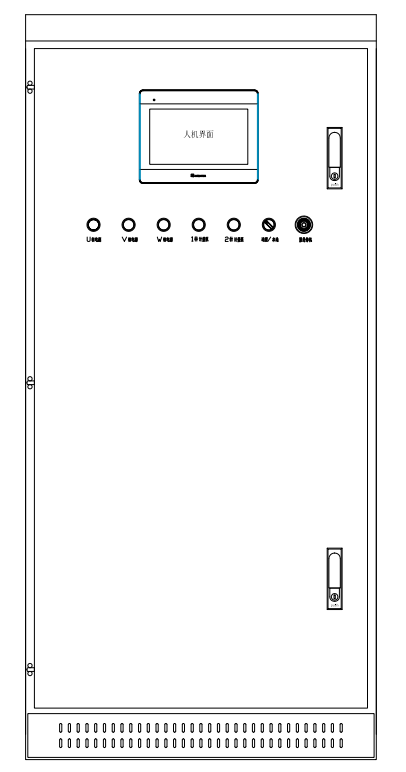
\includegraphics[height=10cm]{g03.PNG}};

                %说明
                \def \itemNumber {1};
                \def \centertPoint {-1.6, 1.8};
                \node at (-2,1.5) (\itemNumber) [text_box] {电柜电源进线指示灯};
                \draw (\centertPoint) rectangle +(1.3,0.5)[red];
                \def \itemNumber {2};
                \def \centertPoint {2,5.5};
                \node at (\centertPoint) (\itemNumber) [text_box] {计量泵运行指示灯};
                \draw [arrow] (\itemNumber) -- (0.3,2);
                \draw (-0.2,1.8) rectangle +(0.7,0.5)[red];
                \def \itemNumber {2};
                \def \centertPoint {0.8, 2.1};
                \node at (1,0) (\itemNumber) [text_box] {远程/在地控制切换};
                \draw [arrow] (\itemNumber) -- (\centertPoint);
                \draw (\centertPoint) circle (0.2)[red];
                \def \itemNumber {3};
                \def \centertPoint {1.3, 2.1};
                \node at (3,1) (\itemNumber) [text_box] {紧急停机按钮};
                \draw [arrow] (\itemNumber) -- (\centertPoint);
                \draw (\centertPoint) circle (0.2)[red];

                % 辅助线
                \def \xLimit {8};
                \def \yLimit {7};
                % 
			% 辅助线
            \draw (-\xLimit,-\yLimit) [help lines] grid (\xLimit,\yLimit);
            \foreach \x in {-\xLimit, ...,\xLimit}{
               \node [red] at (\x, \yLimit) {\x};
               \node [red] at (\x, -\yLimit) {\x};
               \node [red] at (\x, 0) {\x};
            }
            \foreach \y in {-\yLimit, ...,\yLimit}
                  \node [red] at (-\xLimit, \y) {\y};
            \foreach \y in {-\yLimit, ...,\yLimit}
                  \node [red] at (\xLimit, \y) {\y};
            \foreach \y in {-\yLimit, ...,\yLimit}
                  \node [red] at (0, \y) {\y};


            \end{tikzpicture}
            \caption{电柜操作面板布局}\label{fig:p5}
        \end{figure}

